\paragraph{RNN Variants} \label{sec:rnn-variants}

\Acp{RNN} are a class of neural networks designed to handle sequential data. They work by maintaining an internal state or memory, which allows them to process sequences of inputs and produce outputs that depend on previous inputs. This definition allows for other types of networks, different from the one shown in the previous section.

However, there are convincing reasons to investigate architectures beyond the basic approach. The typical \ac{RNN} is not without its difficulties, particularly the development of the \textit{vanishing gradient problem} as a major concern.

\Acp{RNN} may be prone to the vanishing gradient problem due to their method of updating internal states. \Acp{RNN} compute the internal state at time step $t$ by incorporating the input of time step $t$ and the previous state of time step $t-1$. This process generates a sequence of dependencies between the present and past states, which leads to multiple matrix multiplications during the backpropagation.

As the gradient keeps decreasing after each multiplication, it may ultimately shrink to such an extent that the neural network fails to learn long-term patterns present in the input sequence.

The prime example of an architecture that fights the vanishing gradient problem is the \textbf{\acf{LSTM}} \cite{hochreiter_long_1997}. \Acp{LSTM} were introduced in 1997 and have since become a popular choice for processing sequential data, especially in \ac{NLP}.

The main idea behind \ac{LSTM} is to introduce memory cells that can selectively forget or remember information from previous time steps. Each memory cell has three gates: the input gate, the forget gate, and the output gate, which control the flow of information into and out of the cell. One can see how these work in Figure \ref{fig:lstm}.

\begin{figure}[ht]
    \centering
    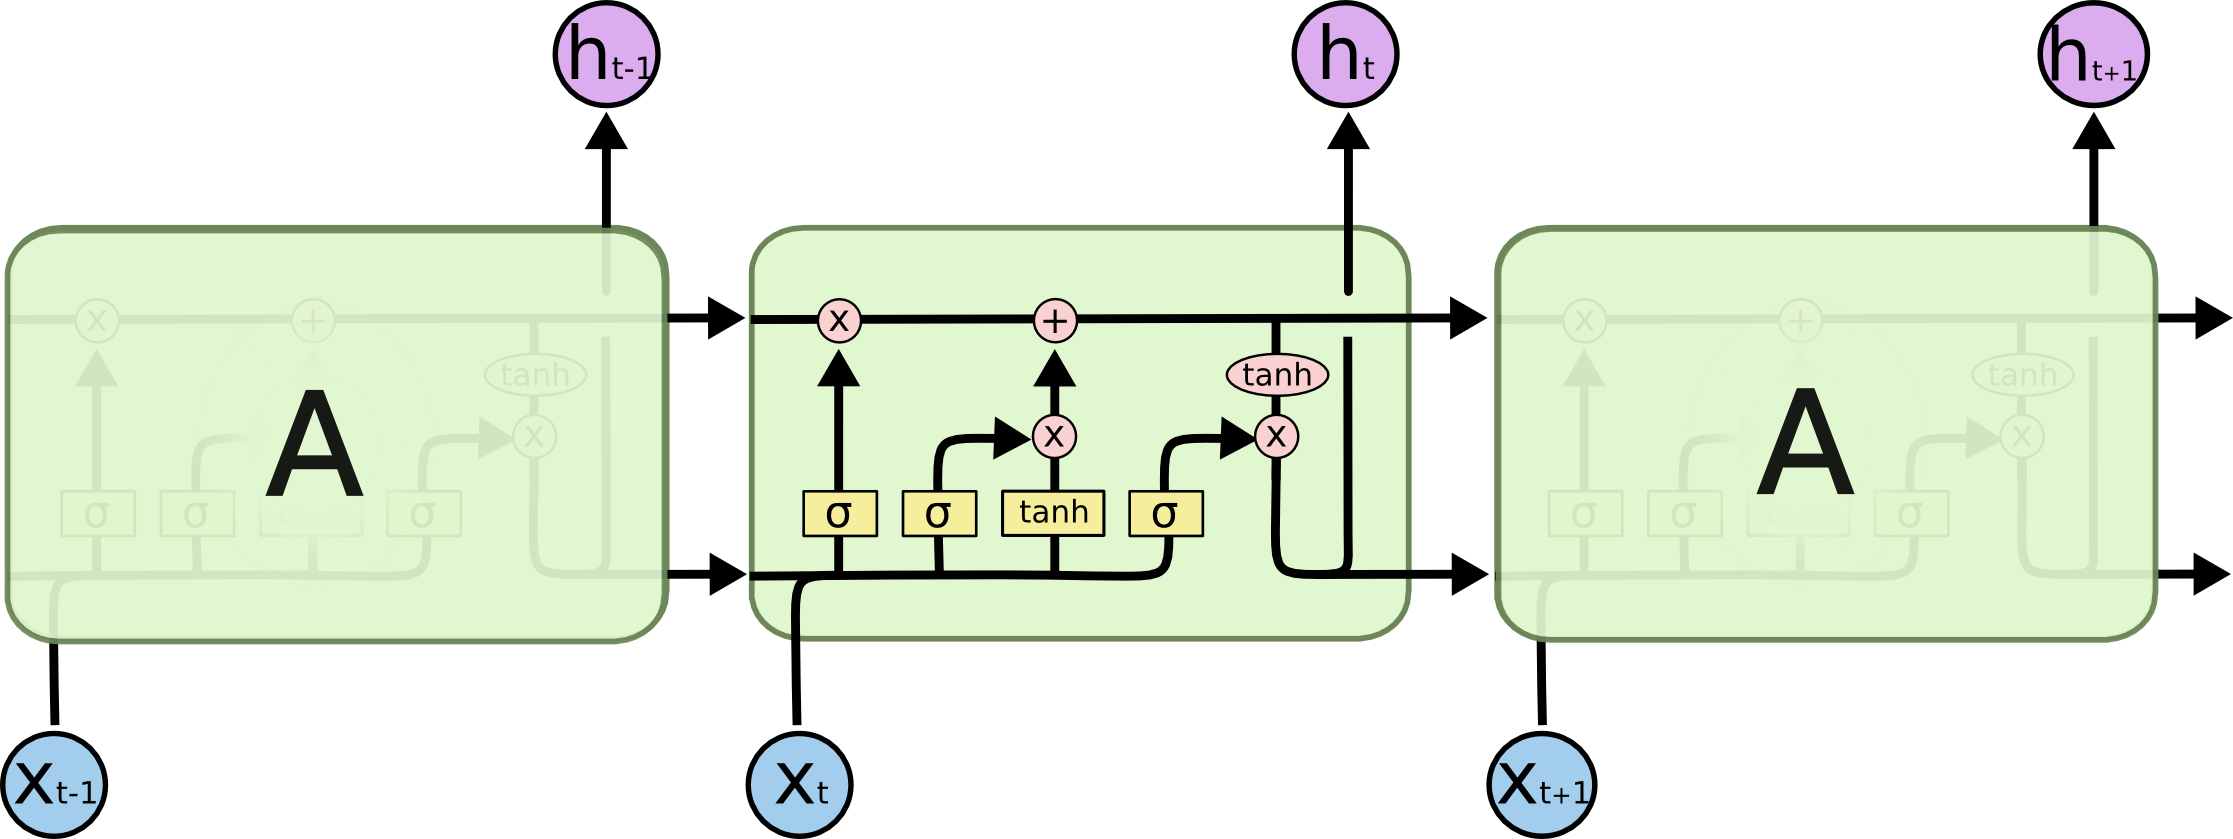
\includegraphics[width=\textwidth]{figures/2-sota/LSTM3-chain.png}
    \caption[Long Short-Term Memory]{\textbf{\Acf{LSTM}} --- 
    The network was taken from \cite{christopher_olah_understanding_2015}. Each green rectangle is an \ac{LSTM} cell. The blue circles represent an input at a given time, such that $X_t$ is the input at time $t$. The pink circles represent the output at a given time $h_t$. Each \ac{LSTM} cell takes three inputs: the previous cell`s memory and output, and the current input, and outputs both the real output and the current memory. In the Figure, the top exiting arrow corresponds to the memory, while the bottom corresponds to the output. The yellow rectangles have learnable parameters, weights, and biases.}
    \label{fig:lstm}
\end{figure}

The forget gate determines which information from the previous state should be forgotten or retained. It takes the current input, $X_t$, and the previous state, $H_{t-1}$, and computes the gate activation, $f_t$, a number between 0 and 1 that determines how much of the previous state should be retained or forgotten. It is calculated as

\begin{equation}
    f_t = \sigma (W_f * [H_{t-1}, X_t] + b_f)    
\end{equation}

$W_f$ is the weight matrix for the forget gate, and $b_f$ is the bias vector.

The input gate determines which information from the current input and the previous state should be allowed into the cell. It takes the current input, $X_t$, and the previous state, $H_{t-1}$, as inputs and computes the gate activation, $i_t$, which is a number between 0 and 1 that determines how much of the input and previous state should be allowed into the cell. It is calculated as

\begin{equation}
    i_t = \sigma (W_i * [H_{t-1}, X_t] + b_i)
\end{equation}

where $\sigma$ is the sigmoid activation function, $W_i$ is the weight matrix for the input gate, and $b_i$ is the bias vector.

The memory update computes the new information stored in the memory cell. It takes the current input, $X_t$, and the previous state, $H_{t-1}$, as inputs and computes the new candidate memory content, $\tilde{C_t}$. It is calculated as

\begin{equation}
    \tilde{C_t} = \tanh (W_C \times [H_{t-1}, X_t] + b_C)
\end{equation}

$W_C$ is the weight matrix for the candidate memory update, and $b_C$ is the bias vector.

The memory cell stores the current memory content, $C_t$, a combination of the previous and new candidate memory content, as determined by the input and forget gates. It is calculated as

\begin{equation}
    C_t = f_t \times C_{t-1} + i_t * \tilde{C_t}
\end{equation}

The output gate determines which information from the current memory cell should be used as output. It takes the current input, $X_t$, and the previous state, $H_{t-1}$, as inputs and computes the gate activation, $o_t$, a number between 0 and 1 that determines how much of the memory cell content should be outputted. It is calculated

\begin{equation}
    o_t = \sigma (W_o \times [H_{t-1}, X_t] + b_o)
\end{equation}

The hidden state, $H_t$, is computed by applying the output gate to the memory cell. It is calculated as

\begin{equation}
    H_t = o_t \times \tanh (C_t)
\end{equation}

By selectively forgetting or remembering information from previous time steps, \acp{LSTM} can maintain long-term dependencies in the input sequence and avoid the vanishing gradient problem that occurs in vanilla \acp{RNN}.

Other kinds of networks that handle the vanishing gradient problem have been proposed. One example is the \textbf{\acf{GRU}}~\cite{cho_learning_2014}. \Ac{GRU} is very similar to \ac{LSTM}. The main difference between \ac{GRU} and \ac{LSTM} is in their architecture and the number of gates they use to control the flow of information. While the \ac{LSTM} has the three gates mentioned above, \ac{GRU} has two gates: the reset gate and the update gate. The update gate controls how much of the previous hidden state to keep, and the reset gate determines how much of the previous hidden state to forget.

Overall, \ac{GRU} has a simpler architecture compared to \ac{LSTM}, which makes it faster to train and requires fewer parameters. However, \ac{LSTM} is generally considered more powerful and better suited for tasks that require longer-term memory, such as machine translation or speech recognition.

Another widespread helpful \ac{RNN} implementation is the \textbf{bidirectional \ac{RNN}}~\cite{schuster_bidirectional_1997}. Unlike traditional \acp{RNN}, which process input sequences in only one direction, from beginning to end, bidirectional \acp{RNN} process input sequences in both directions, from beginning to end and from end to beginning, simultaneously.

The main idea behind bidirectional \acp{RNN} is to use two separate \acp{RNN}, one that reads the input sequence in the forward direction and another that reads the sequence in the backward direction. The output of the two \acp{RNN} are then combined to produce the final output.

The benefit of using a bidirectional \ac{RNN} is that it allows the network to access both past and future context when making predictions about the current time step.